\documentclass{article}
\usepackage[utf8]{inputenc}

\title{Quicksort}
\author{Manuel Serna-Aguilera}
\date{}
\setlength{\parindent}{0pt}

\usepackage{natbib}
\usepackage{graphicx}
\usepackage{amsmath}
\usepackage{clrscode3e}

\begin{document}

\maketitle

\section*{Introduction}
% section 7.1 content with all 3 figures added
Quicksort is a very popular sorting algorithm, despite its worst-case running time being $\Theta{(n^2)}$, it is nonetheless very effecient on average with an expected running time of $\Theta{(n \cdot \log_2(n))}$. The constant factors hidden by the asymptotic notation are small. Assuming distinct input elements, its expected running time is $O{(n \cdot \log_2(n))}$.
\\ \\
Like merge sort, quicksort utilizes the divide-and-conquer paradigm, taking in an array $A[p \twodots r]$, it performs the following steps.
\begin{itemize}
    \item[] \textbf{Divide}: Partition (rearrange) the array $A[p \twodots r]$ into two (possibly empty) subarrays $A[p \twodots q-1]$ and $A[q+1 \twodots r]$ such that each element of $A[p \twodots q-1]$ is less than or equal to $A[q]$, which is, in turn, less than or equal to each element of $A[q+1 \twodots r]$. Compute the index $q$ as part of this partitioning procedure (this can be a simple or complex process).
    \item[] \textbf{Conquer}: Sort the two subarrays $A[p \twodots q-1]$ and $A[q+1 \twodots r]$ by recursive calls to quicksort.
    \item[] \textbf{Combine}: The subarrays are already sorted, and no work is needed to combine them (as quicksort sorts in place).
\end{itemize}

\newpage

Here are the procedures for quicksort.

\begin{codebox}
\Procname{\proc{quicksort}$(A, p, r)$}
\li \If $p < r$
\li \Then
        $q = \proc{partition}(A, p, r)$
\li     $\proc{quicksort}(A, p, q-1)$
\li     $\proc{quicksort}(A, q+1, r)$
    \End
\end{codebox}

To sort an entire array $A$, the initial call is $\proc{quicksort}(A, 1, \attrib{A}{length})$.

\begin{codebox}
\Procname{\proc{partition}$(A, p, r)$}
\li $x = A[r]$ \Comment this partition procedure always picks the right-most element 
\li $i = p-1$
\li \For $j \gets p$ \To $r-1$
    \Do
\li     \If $A[j] \leq x$
            \Then
\li             $i = i + 1$
\li             exchange $A[i]$ with $A[j]$
            \End
    \End
\li exchange $A[i+1]$ with $A[r]$
\li \Return $i + 1$
\end{codebox}

Figure 1 shows how the partition procedure works on an example 8-element array. This particular partition picks the right-most element in the subarray as its \textbf{pivot}, which is how we divide the subarrays; note that we can have any index be the partition, the book just does it this way for simplicity.

% figure 7.1
\begin{figure}[!ht]
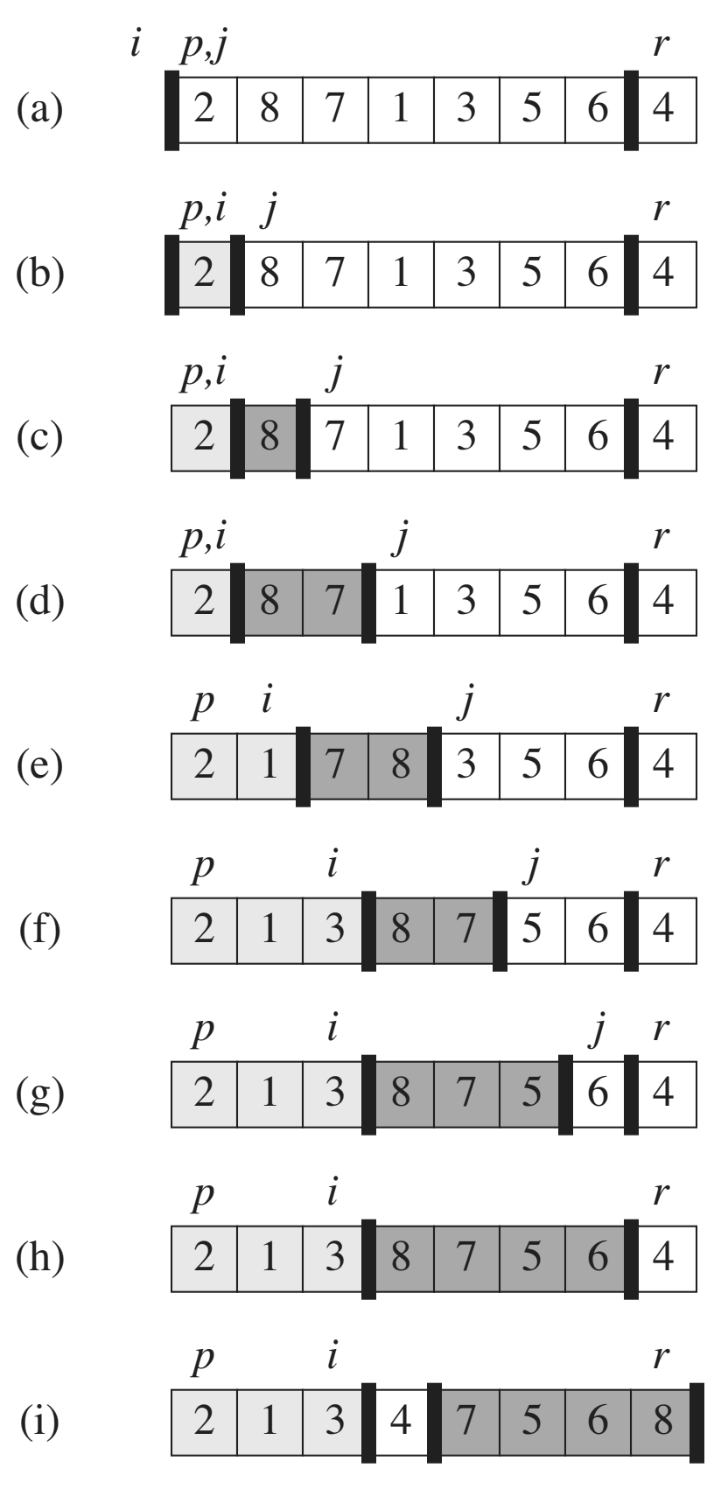
\includegraphics[scale=0.45]{quicksort_example}
\caption{
    A visual example of the process of partition. Array entry $A[r]$ becomes the pivot element $x$. Lightly shaded array elements are all in the first partition with values no greater than $x$. Heavily shaded elements are in the second partition with values greater than $x$. The unshaded elements have not yet been put in one of the first two partitions, and the final white element is the pivot $x$. 
    \textbf{(a)} The initial array and variable settings. None of the elements have been placed in either of the first two partitions.
    \textbf{(b)} The value 2 is “swapped with itself” and put in the partition of smaller values. 
    \textbf{(c)–(d)} The values 8 and 7 are added to the partition of larger values. 
    \textbf{(e)} The values 1 and 8 are swapped, and the smaller partition grows. 
    \textbf{(f)}The values 3 and 7 are swapped, and the smaller partition grows. 
    \textbf{(g)–(h)} The larger partition grows to include 5 and 6, and the loop terminates. 
    \textbf{(i)} In lines 7–8, the pivot element is swapped so that it lies between the two partitions.
}
\label{fig:quicksort1}
\end{figure}

\clearpage

% figure 7.2
\begin{figure}[!ht]
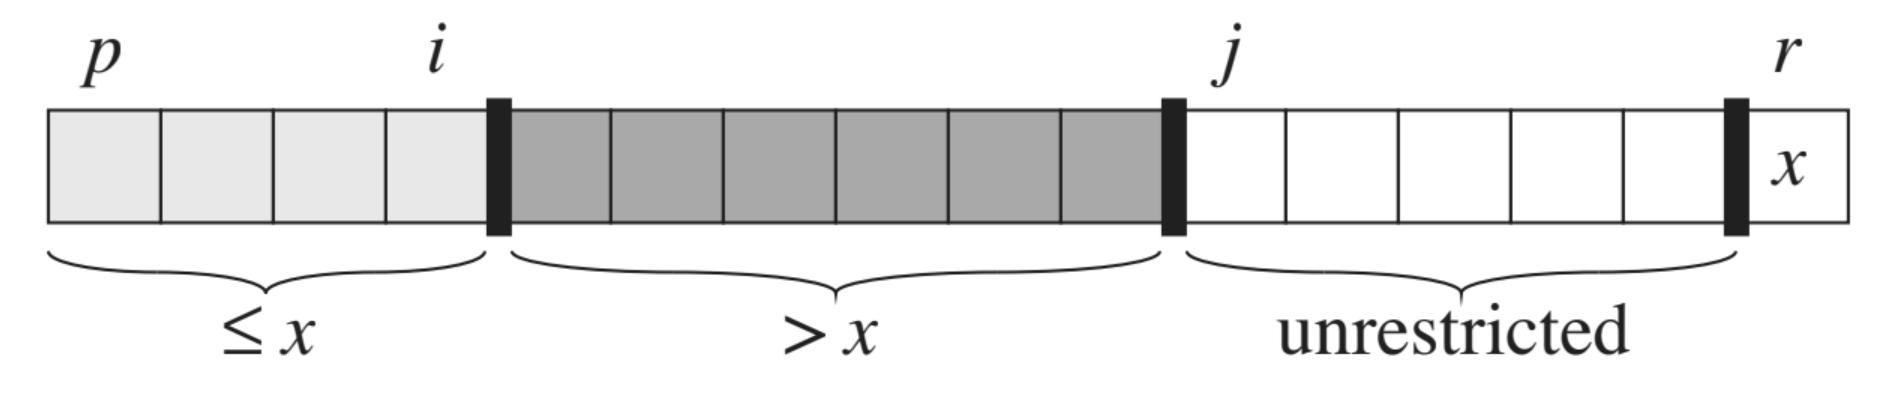
\includegraphics[scale=0.25]{partitions}
\caption{
    The four regions maintained by the procedure $\proc{partition}$ on a subarray $A[p \twodots r]$. The values in $A[p \twodots i]$ are all less than or equal to $x$, the values in $A[i+1 \twodots j-1]$ are all greater than x, and $A[r] = x$. The subarray $A[p \twodots r-1]$ can take on any values.
}
\label{fig:quicksort2}
\end{figure}

% figure 7.3
\begin{figure}[!ht]
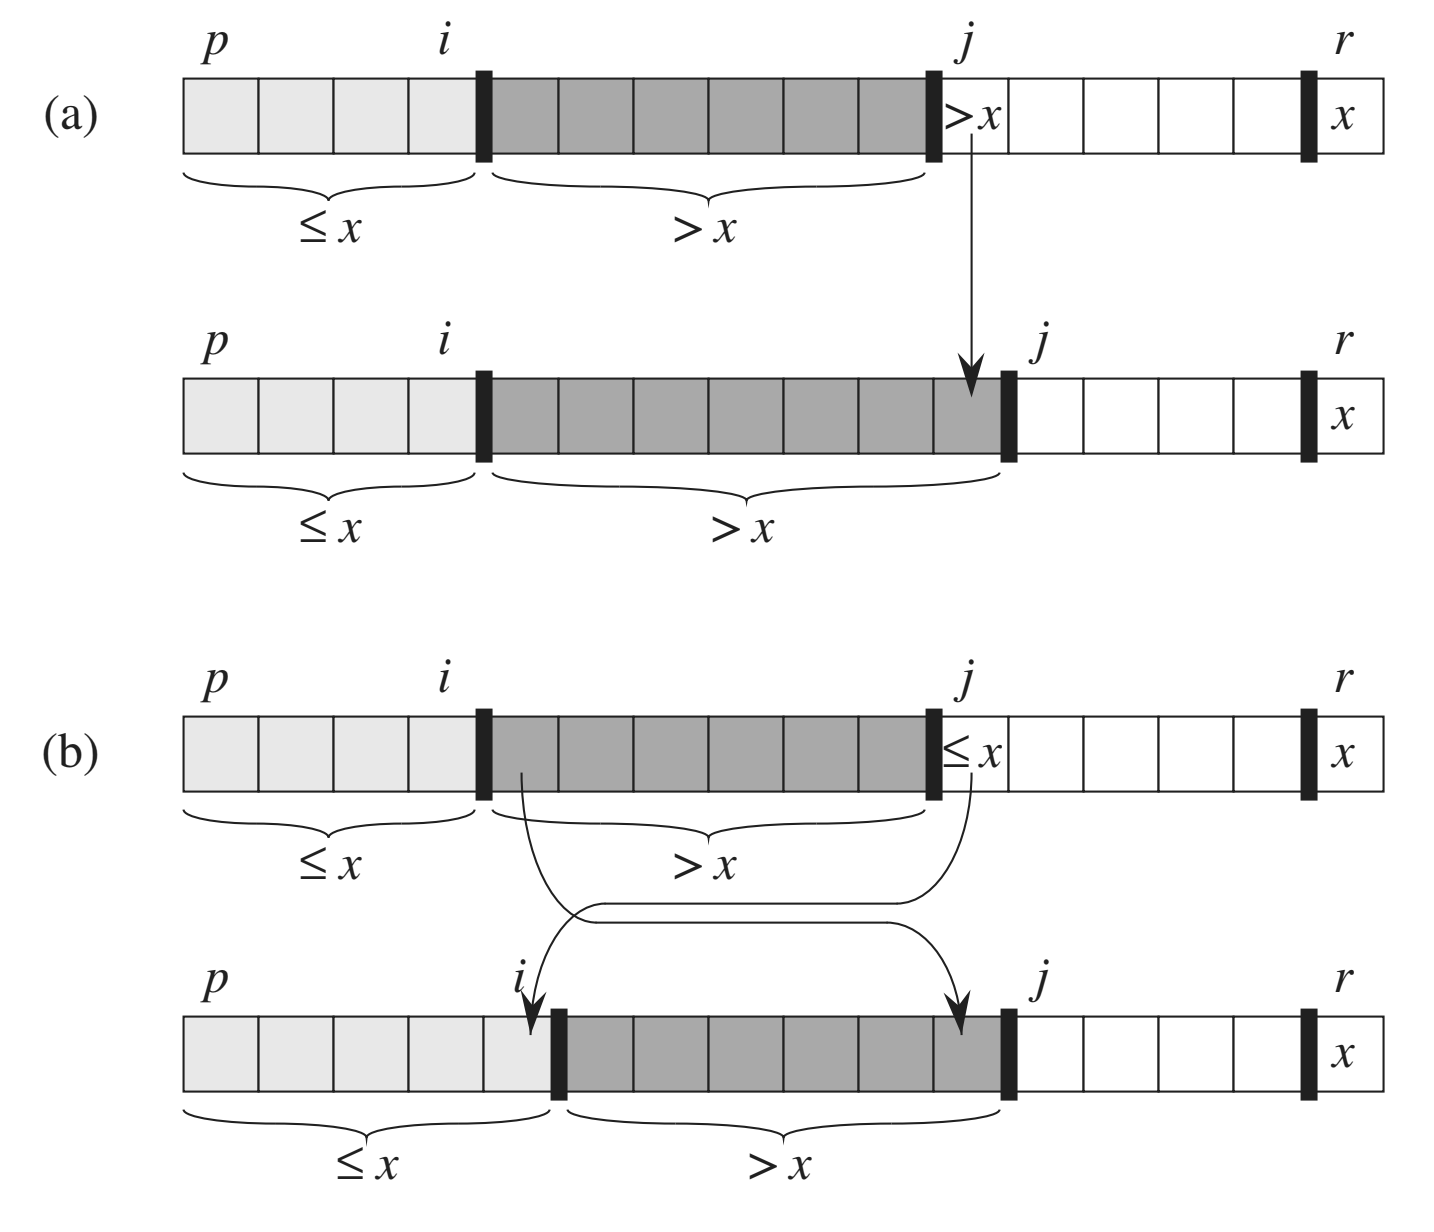
\includegraphics[scale=0.45]{partition_cases}
\caption{
    The two cases for one iteration of procedure $\proc{partition}$. 
    \textbf{(a)} If $A[j] > x$, the only action is to increment $j$.
    \textbf{(b)} If $A[j] \leq x$, index $i$ is incremented, $A[i]$ and $A[j]$ are swapped, and then $j$ is incremented.
}
\label{fig:quicksort3}
\end{figure}

\newpage

\section*{Performance}
The \textbf{best case} of quicksort occurs when $\proc{partition}$ evenly splits the array every time it is called. The actual sizes of the splits are $\lfloor n/2 \rfloor$ and $\lfloor n/2 \rfloor - 1$ since we do not include the partition value when we recurse. Even so, we can simplify the sizes to be the same since the time cost will pretty much be the same. This ideal situation gives the recurrence

\begin{equation*}
    T(n) = 2T(n/2) + cn + 1.
\end{equation*}

By the master method,

\begin{equation*}
\begin{split}
    n^{\log_b{a}} & = n^{\log_2{2}} = n^1 \\
    f(n) & = cn = \theta{(n)}. \text{\hspace{10mm}(case 2)}
\end{split}
\end{equation*}
\\
Thus, the closed-form solution and the best-case running time for quicksort is
\begin{equation*}
    T(n) = \Theta{(n \cdot \log_2{(n)})}.
\end{equation*}
\\
The \textbf{worst case} of quicksort occurs when the array is already sorted in increasing order, giving the following recurrence.

\begin{equation*}
\begin{split}
    T(n) &= T(n-1) + cn \\
        &= T(n-i) + i \cdot cn\\
    & \hspace{35mm} n - i = 1 \text{ (aside)}\\
    & \hspace{35mm} n - 1 + i \\
    & \hspace{35mm} T(1) = c \\
        &= T(1) + cn(n-1)\\
        &= 1 + cn^{2} - cn\\
        &= cn^{2} - cn + 1\\
    T(n) &= \Theta{(n^2)} \text{ is our closed-form solution and worst-case running time.}
\end{split}
\end{equation*}

\end{document}
